% This is samplepaper.tex, a sample chapter demonstrating the
% LLNCS macro package for Springer Computer Science proceedings;
% Version 2.21 of 2022/01/12
%
\documentclass[runningheads]{llncs}
%
\usepackage[T1]{fontenc}
% T1 fonts will be used to generate the final print and online PDFs,
% so please use T1 fonts in your manuscript whenever possible.
% Other font encondings may result in incorrect characters.
%
\usepackage{graphicx}
% Used for displaying a sample figure. If possible, figure files should
% be included in EPS format.
%
% If you use the hyperref package, please uncomment the following two lines
% to display URLs in blue roman font according to Springer's eBook style:
%\renewcommand\UrlFont{\color{blue}\rmfamily}
%
\usepackage{orcidlink}

%\usepackage[backend=biber,style=numeric,sortcites,sorting=nty,backref,natbib,hyperref]{biblatex}

%\addbibresource{ref.bib}
\usepackage{float}
\usepackage{booktabs}
\usepackage{arydshln}
\usepackage{amsmath}

\usepackage{pgfplots}
\pgfplotsset{compat=1.17}
\begin{document}
%
\title{Optimal Frequency Regularization: Decrease the Usage of Random Access Memory on Android Devices\thanks{Supported by University of Alberta.}}
%
%\titlerunning{Abbreviated paper title}
% If the paper title is too long for the running head, you can set
% an abbreviated paper title here
%
\author{Wenhao You\inst{1}\orcidlink{0009-0008-3267-5674} \and
Leo Chang\inst{2}\orcidlink{0009-0006-1497-7279} \and
Guanfang Dong\inst{3}\orcidlink{0000-0001-9300-2125} \and
Anup Basu\inst{4}\orcidlink{0000-0002-7695-4148}}
%
\authorrunning{W. You et al.}
% First names are abbreviated in the running head.
% If there are more than two authors, 'et al.' is used.
%
\institute{
University of Alberta, Edmonton, Canada\\
\email{\{wyou1,chewei\}@ualberta.ca}}
%
\maketitle              % typeset the header of the contribution
%
\begin{abstract}
We implemented Frequency Regularization on Android devices successfully and packaged FR into a Python library that can be successfully deployed on Android devices as well. Moreover, we proposed an optimal version of FR to reduce usage or random access memory. We used Android Studio to develop software containing FR and utilized Termux for deploying our FR Python library on mobile devices. Additionally, for the optimal version of FR, we adopted a layer-by-layer memory freeing approach to optimize FR, and we divided a complete image into four different parts for separated FR processing. Our experiments showed that the layer-by-layer memory freeing method significantly reduced the usage of random access memory on Android devices. It makes an increasingly possible for low-end hardware mobile devices to deploy certain useful and complex neural networks.

\keywords{Frequency regularization  \and Optimal frequency regularization \and Python library \and Random access memory \and Android devices.}
\end{abstract}
%
%
%
\section{Introduction}

Currently, people can not live without mobile devices. These compact yet powerful gadgets have become indispensable tools for communication, entertainment, and information. Their portability and versatility make them a constant companion. Meanwhile, Convolutional neural networks play an important role in computer vision applications. However, these neural networks are usually implemented on high-specification hardware. There are several advantages of running convolutional neural networks on mobile devices: privacy, internet, and runtime. For enhancing privacy, personal information does not need to be uploaded or transmitted to the cloud servers anymore. For reading the dependence on the internet connection, the functionality on local devices can replace some internet services. For the runtime, especially some applications that need real-time feedback, without connecting to the cloud server can shorten the processing time. In all, convolutional neural networks can totally replace the usage of many applications on mobile devices, ensuring personal data security. 

According to the popularity of mobile devices and the benefits of convolutional neural networks, we want to find a way to deploy some large and complex convolutional neural networks on mobile devices, leading to the question: “How can we deploy large convolutional neural networks on mobile devices?”

We found five methods to achieve our goal: upgrade the hardware of mobile devices; use Extreme Learning Machine (ELM)~\cite{anton2021elm} to allocate the weight of the hidden layers randomly in order to train large models on mobile devices faster; use NestDNN~\cite{fang2018nestdnn} dynamically adjust the size and computational complexity of the network based on available resources on mobile devices; use “One-shot Whole Network Compression”~\cite{kim2016oneshot} to prune, quantize, and compress the neural networks; use Frequency Regularization (FR)~\cite{zhao2023fr} to reduce parameters by removing high-frequency component. We make a more detailed introduction to their drawbacks and limitations in Section~\ref{related_work}.

After conducting a thorough literature review, considering all the limitations, accuracy, complexity, and future potential, we choose Frequency Regularization (FR) as our target algorithm, deploying it on one of the most popular mobile devices - Android mobile. Our main idea uses FR to compress a convolutional neural network U-Net and then decompresses the uploaded compressed model on an Android mobile device in a short time. After that, use the decompressed model to do image segmentation for the Carvana Image Masking Challenge Dataset~\cite{brian2017carvanadataset}. 

\begin{figure}[htbp]
	\centering
	\label{image:workflow}
	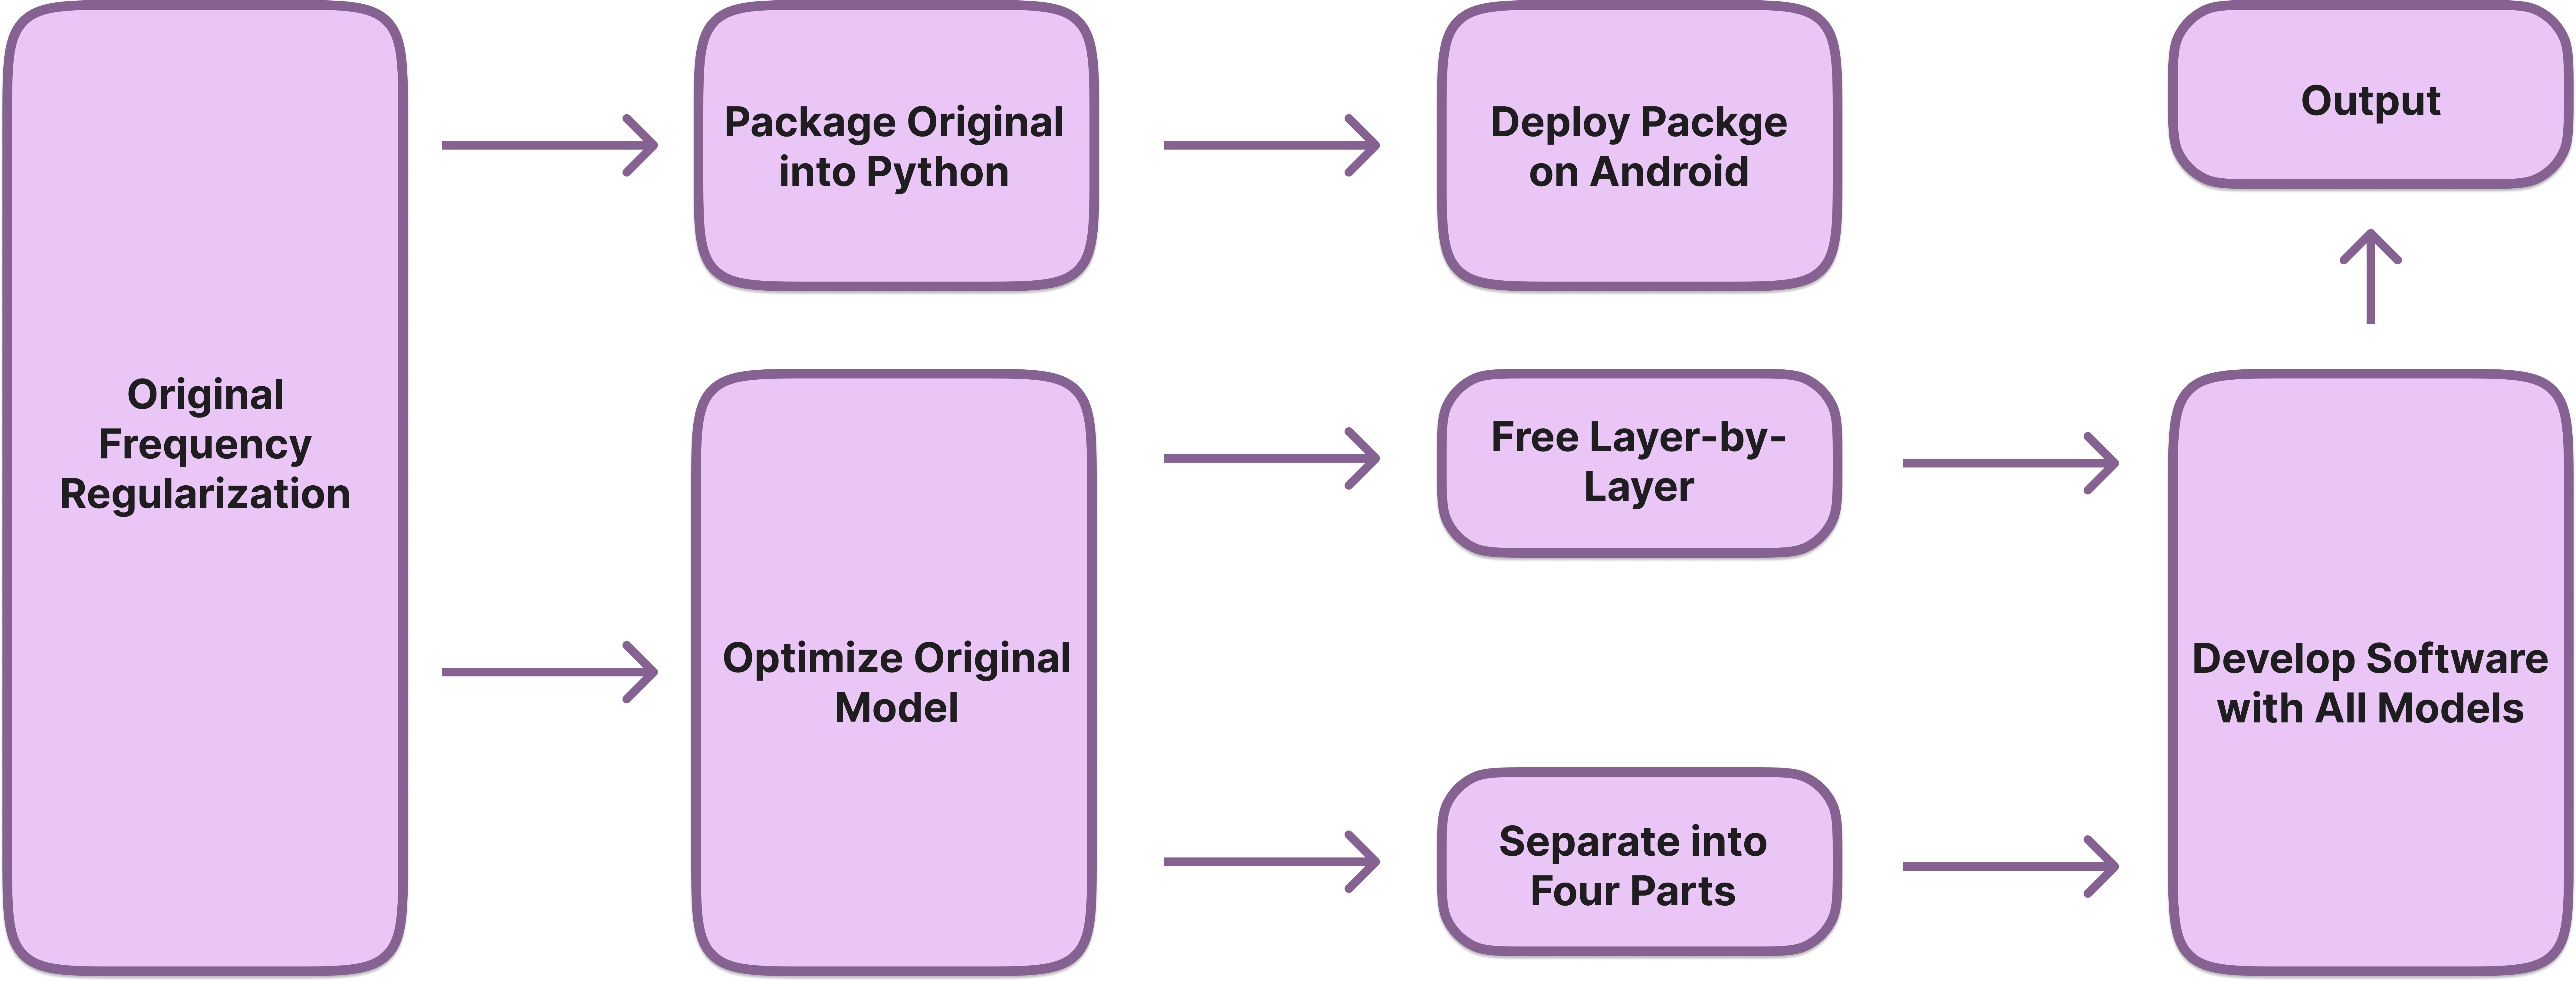
\includegraphics[width=1\linewidth]{figures/workflow.jpg}
	\caption{General workflow of deploying frequency regularization and its optimal versions on Android devices.}
\end{figure}

In our work, before optimize the existing FR code~\cite{fr_repo} on Android, we have two different directions to go. One is to deploy the Linux environment by using Termux~\cite{termux_repo},~\cite{termux_overview},~\cite{termux_wiki} on the Android system and to realize the source code implementation. Another one is to develop Android software which contains frequency regularization by using Android Studio. As shown in Fig.~\ref{image:workflow}, our workflow also contains the optimization/improvement of existing frequency regularization~\cite{zhao2023fr},~\cite{fr_repo}. The approach of freeing RAM layer-by-layer does decrease the total usage of RAM on Android phones significantly and the quality of the image segmentation does not have any side effects. Overall, our main contributions are:\\
1. Packing a Python library of frequency regularization and installing it on the Android system successfully.\\
2. Optimizing and improving the existing frequency regularization, decresing the usage of RAM on Android devices.\\
3. Developing Android software containing original frequency regularization and all the other optimal versions to do image segmentation.

Our optimal models achieve the usage of RAM around 1.9318 GB and the usage of RAM by using original frequency regularization is around 3.2697 GB on Android devices. This means the optimal models are  40.9\% relative improvements over previous algorithm~\cite{zhao2023fr},~\cite{fr_repo} specially for Android devices.



\section{Related Work}\label{related_work}

Extreme learning machine (ELM) has been widely used in artificial intelligence field over the last decades~\cite{anton2021elm},~\cite{ding2014elmapp},~\cite{wang2022elmapp},~\cite{deng2015elmapp},~\cite{huang2006elmapp}. Although this algorithm has seen significant development, it also has several drawbacks: 
\begin{itemize}
	\item Poor tunability: It has poor controllability of the model since ELM calculates the least squares solution directly, and users cannot analyze the characteristics of the datasets to fine-tune. Adjusting models based on specific performance of mobile devices is important to mobile development.
	\item Lack of robustness: The performance of the model can be affected significantly while including certain outliers in different datasets, indicating poor robustness. Deployment on mobile devices needs to handle various inputs, including every potential outlier. Although there are many advanced versions of ELM~\cite{john2015advancedelm},~\cite{zhang2015advancedelm},~\cite{zhu2005advancedelm},~\cite{sun2017advancedelm} they lacks universality and are not as easy as other algorithms to deploy.
	\item Overfitting issues: While deploying large convolutional neural networks on mobile devices, model generalization is crucial since overfitting can result in poor performance on unseen data. ELM easily leads to overfitting issues because it is based on empirical risk minimization without considering structural risk. Xue et al.~\cite{ying2019overfit}pointed to a regularization strategy to solve this problem by feature-selection.
\end{itemize}	 

NestDNN is a framework that takes the dynamics of runtime resources into account~\cite{fang2018nestdnn}. The experiment of Fang et al.~\cite{fang2018nestdnn} achieves as much as 4.2\% increase in inference accuracy, 2.0× increase in video frame processing rate and 1.7× reduction in energy consumption. However, NestDNN also comes with some limitations. Its computational cost is significantly higher by using filter pruning method Triplet Response Residual (TRR). The high computational cost could probably exceed the processing capabilities of existing mobile devices and the runtime of model generation may be too long, which is not suitable for our deployment. 

``One-shot Whole Network Compression"~\cite{kim2016oneshot} includes removing certain parameters or structures, which is irreversible. Moreover, by using this compression method, the accuracy is too low. For example, in the experiment of Kim et al., by using AlexNet, the accuracy of the compressed model can drop by more than 50\%. In order to increase its accuracy, we have to fine-tune the compressed model. Increasing accuracy requires at least more than 10 training epochs, which wastes too much time. In our work, to deploy on mobile devices, this algorithm can not be chosen obviously. 

The proposed frequency regularization (FR)~\cite{zhao2023fr} works by restricting the non-zero elements of network parameters in the frequency domain, thus reducing information redundancy. Table~\ref{table:fr_unet} illustrates the evaluation of the proposed frequency regularization on UNet, according to compression rate, number of parameters, and dice score. Dice score is a metric for assessing the quality of image segmentation and ranges from 0 to 1, where 0 indicates no overlap and 1 indicates perfect overlap. The data under the dashed line represents the result under the most extreme condition in which only 759 float16 parameters are kept in UNet-v4. Thus, according to the surprised and satisfying experiment outcomes, we choose the frequency regularization as our compression method, to deploy it on mobile devices (i.e. Android system).

\begin{table}[H]
	\caption{Evaluation of the proposed frequency regularization on UNet for image segmentation tasks using Carvana Image Masking Challenge Dataset~\cite{zhao2023fr},~\cite{brian2017carvanadataset}.} 
	\label{table:fr_unet}
	\small
	\centering
	\begin{tabular}{rrrr}
		\toprule
		&Dice Score&Compression Rate&\# of Parameters\\ 
		\midrule\midrule
		UNet-ref&99.13\%&100\%(1×)&31,043,586\\
		UNet-v1&99.51\%&1\%(100×)&310,964\\
		UNet-v2&99.37\%&0.1\%(1000×)&31,096\\
		UNet-v3&98.86\%&0.0094\%(10573×)&2,936\\
		\cdashline{1-4}
		UNet-v4&97.19\%&0.0012\%(81801×)&759(float16)\\
		\bottomrule
	\end{tabular}
\end{table}

\section{Methodology}\label{methodology}
\subsection{Problem Formulation}~\label{formulation}
To deploy frequency regularization on mobile devices, we have to handle the limited hardware of mobile devices. Our main problem which needs to be solved is to decrease the memory usage while keeping the quality of the image as much as possible.

\subsection{Original and Optimal Versions of Frequency Regularization}~\label{optimal}
To carry out the experiment of image segmentation, we designed two creative methods based on Frequency Regularization to optimize the usage of memory and its efficiency. 
\begin{itemize}
	\item Original frequency regularization: In Section~\ref{related_work}, Zhao et al. designed this method and we will use their source code~\cite{fr_repo} to implement it on Android system.
	\item Free random access memory layer by layer based on frequency regularization: For this optimal method, we store the information of the whole network layer by layer and free the random access memory (RAM) while each layer ends. 
	\item Free random access memory layer by layer based on frequency regularization and seperate one image into four parts: The main idea is same to the previous method. On this method, we plan to sepearte a image into four different parts and implement the previous method upon each four parts independently. After that, we merge the four parts together to get the result. 
\end{itemize}	 		

\subsection{Deployment Tools}~\label{deployment}
To deploy all the Frequency Regularization related methods in Section~\ref{optimal} on Android devices, we have two tools to use. One is Termux, which can implement a Linux environment on an Android system. Another one is Android Studio, which can help to develop Apps with FR image segmentation.
\begin{itemize}
	\item Termux: Termux~\cite{termux_repo},~\cite{termux_overview},~\cite{termux_wiki}  is an Android terminal application and Linux environment. It works directly with no rooting or setup required. To use Termux, the system needs to meet some requirements: Android 5.0 - 12.0; CPU: AArch64, ARM, i686, x86\_64; at least 300 MB of disk space. It is open source and can be accessed at https://github.com/termux/termux-app. The instruction of deploy Termux on Android devices is available at https://github.com/btxcy/NeuralOnMobile\#readme. 
	\item Android Studio: Android Studio is an Integrated Development Environment (IDE) designed specifically for developing applications for the Android platform. Moreover, this platform fits the PyTorch Mobile Library very well, which is easy to develop with neural networks.
\end{itemize}	 		

\subsection{Qualitative and Quantitative Metrics}~\label{metrics}
To analyze the results of our experiment, we have three qualitative and quantitative metrices: usage of random access memory, dice score, and visual perception.
\begin{itemize}
	\item Usage of Random Access Memory (RAM): The usage of RAM is a key metric when evaluating the performance of any software application. RAM usage usually refers to the amount of memory that the system allocates to a particular task or application while it is running. This quantitative metric reflects the demand for computing resources, as well as its efficiency. The lower usage of RAM an application uses, the higher efficiency the application has. In Section~\ref{experiments}, we tried to decrease the usage of RAM in order to avoid unnecessary waste of resources and allow more Android devices with lower-end hardware to implement the neural networks.
	% As we run the algorithm on mobile devices, the compressing algorithm Frequency Regularization becomes more significant in this experiment. Mobile device manufacturers increase their memory storage and CPUs to highlight their performance. There are some methods we implemented during the research to compress memory usage. For instance, when running the U-Net neural network layers, saving the outputs in the local storage helps to decrease memory usage. The reason is that output tensors from each layer contain large sizes to store in the memory. But by saving them locally, we can instantly free the memory without occupying it. The next layer can easily access the tensors from the local storage instead of the memory. It helps to reduce about two gigabytes of random memory usage. There is another method to reduce memory usage. As the algorithm requires more memory than the original neural network model from PyTorch, we can make the Frequency Regularization algorithm run only once when initializing the neural network. However, the method does not have a dramatic decrease in memory usage as the previous method. 
	\item Dice Score: It is also known as the Dice Similarity Coefficient. It is a measure of the similarity between two sets of data, usually represented as binary arrays~\cite{dicescore2023}. For example, in the image segmentation of Section~\ref{experiments}, the dice score can be used to evaluate the similarity between a predicted segmentation mask and the ground truth segmentation mask~\cite{dicescore2023}. Its range is 0 to 1, representing no overlap to perfect overlap. We used this quantitative metirc to evaluation the performance of the algorithms. Equation \eqref{eq:dice} shows the formula of dice score~\cite{yerram2020dice}.
	
	\begin{equation}\label{eq:dice}
		\text{Dice Score} = \frac{2 \times |X \cap Y|}{|X| + |Y|}
	\end{equation}
\\where X is the predicted set of pixels and Y is the ground truth.
	\item Visual Perception: Visual perception as a metric in image quality assessment involves evaluating images based on how well they align with human visual characteristics~\cite{fu2016visual}. Though numerous image quality measures have been proposed, human visual perception is still a good way to evaluate the quility of images~\cite{wajid2014visual}. In all, we used our own perception as qalitative metirc and combined with the other two quantative metrics to decide the best outcomes in our experiment. 
\end{itemize}	



\section{Experiments} ~\label{experiments}
\subsection{Experimental Settings}
We utilized an Android device which ran version 12.0.1 for this section. In order to facilitate the deployment of an Ubuntu environment within the Android system, we downloaded Termux~\cite{termux_repo},~\cite{termux_overview},~\cite{termux_wiki}, which version is v0.118.0. Upon accessing Termux, we employed a suite of basic tools, such as wget, proot, and git, to establish the Ubuntu environment. The Ubuntu package~\cite{ubuntu_in_termux_repo} we used is quite different from the conventional Ubuntu installations on normal personal computers. For more detailed steps of setting up the environment, please check our source code repository~\cite{nerual_on_mobile_repo}. For developing the Android Application, we utilized the same version of the Android emulator and made sure that the Android Studio we chose is 2023.1.1. The more detailed steps can be checked on our source code repository as well~\cite{nerual_on_mobile_repo}.


\subsection{Package Frequency Regularization Source Code}~\label{package_fr}
As current and future plans of Zhao et al.~\cite{fr_repo},~\cite{zhao2023fr}, we have accomplished the development of a pip repository for their Frequency Regularization technique and committed to their original repository. We can now integrate Frequency Regularization into our project by simply running the command line in Linux environment: \texttt{\$ pip install frereg}. This step is instrumental in simplifying the deployment of condensed yet potent models in pragmatic applications. We will use this python library in Section~\ref{build_linux}.

\subsection{Build Linux Environment and Install the Frequency Regularization Library} ~\label{build_linux}
After initiating the Ubuntu environment and installing both Python and the Python-pip tool, we used the command line we mentioned in Section~\ref{package_fr}, installing the frequency regularization project successfully. From our own perspectives, this method is not that innovative since it is based on the Termux, which is a mature Linux environment for Android system. This part of our experiment aims to prove the possibility of running a compressed model by building a Linux environment, that only needs enough RAM.


\subsection{Develop an Application with Optimal Methods}~\label{deploy_as}
As mentioned in Section~\ref{methodology}, we utilize Android Studio to develop an application with our methods. In order to run the Python script on the Android Studio, there is a Python library called Chaquopy~\cite{chaquopy2023} that can help us. Our Android application can upload the chosen images from local storage and implement the original Frequency Regularization or the other optimal methods respectively. We use this application to generate all the data we need in this research, such as the usage of RAM. We show the outputs from the algorithm running on an Android phone by making an application using Android Studio to run the Frequency Regularization. The only feature the application provides currently is importing the images from the local machine directory. After that, we get the output from the compressed neural network. 


\begin{table}[H]
	\caption{Comparison of Usages of RAM for Image Segmentation for Carvana Image Masking Challenge Dataset~\cite{brian2017carvanadataset} on an Android Phone: Original FR, Free RAM Layer by Layer FR, and Free RAM Layer by Layer FR with Four Different Parts in Section~\ref{methodology}.} 
	\label{table:ram_usage}
	\small
	\centering
		    \setlength{\tabcolsep}{10pt}
	\begin{tabular}{rrrr}
		\toprule
		& Original & Free Layer & Free Layer (4-parts)\\
		\midrule\midrule
		1$^{st}$ Avg.&3.4088 GB&2.0217 GB&1.2684 GB\\
		2$^{nd}$ Avg.&3.1013 GB&1.8294 GB&1.2602 GB\\
		3$^{rd}$ Avg.&3.2959 GB&1.9444 GB&1.3823 GB\\
		\cdashline{1-4}
		Total Avg.&3.2687 GB&1.9318 GB&1.3036 GB\\
		\bottomrule
	\end{tabular}
\end{table}

\begin{table}[H]
	\caption{Comparison of Dice Scores for Image Segmentation for Carvana Image Masking Challenge Dataset~\cite{brian2017carvanadataset} on an Android Phone: Original FR, Free RAM Layer by Layer FR, and Free RAM Layer by Layer FR with Four Different Parts in Section~\ref{methodology}.} 
	\label{table:dice_score}
	\small
	\centering
	    \setlength{\tabcolsep}{10pt}
\begin{tabular}{rrrr}
	\toprule
	& Original & Free Layer & Free Layer (4-parts)\\
	\midrule\midrule
	1$^{st}$ Avg.&0.9718&0.9718&0.7567\\
	2$^{nd}$ Avg.&0.9718&0.9718&0.7567\\
	3$^{rd}$ Avg.&0.9718&0.9718&0.7567\\
	\cdashline{1-4}
	Total Avg.&0.9718&0.9718&0.7567\\
	\bottomrule
\end{tabular}
\end{table}

\begin{figure}[htbp]
	\centering
	\label{image:3_outputs}
	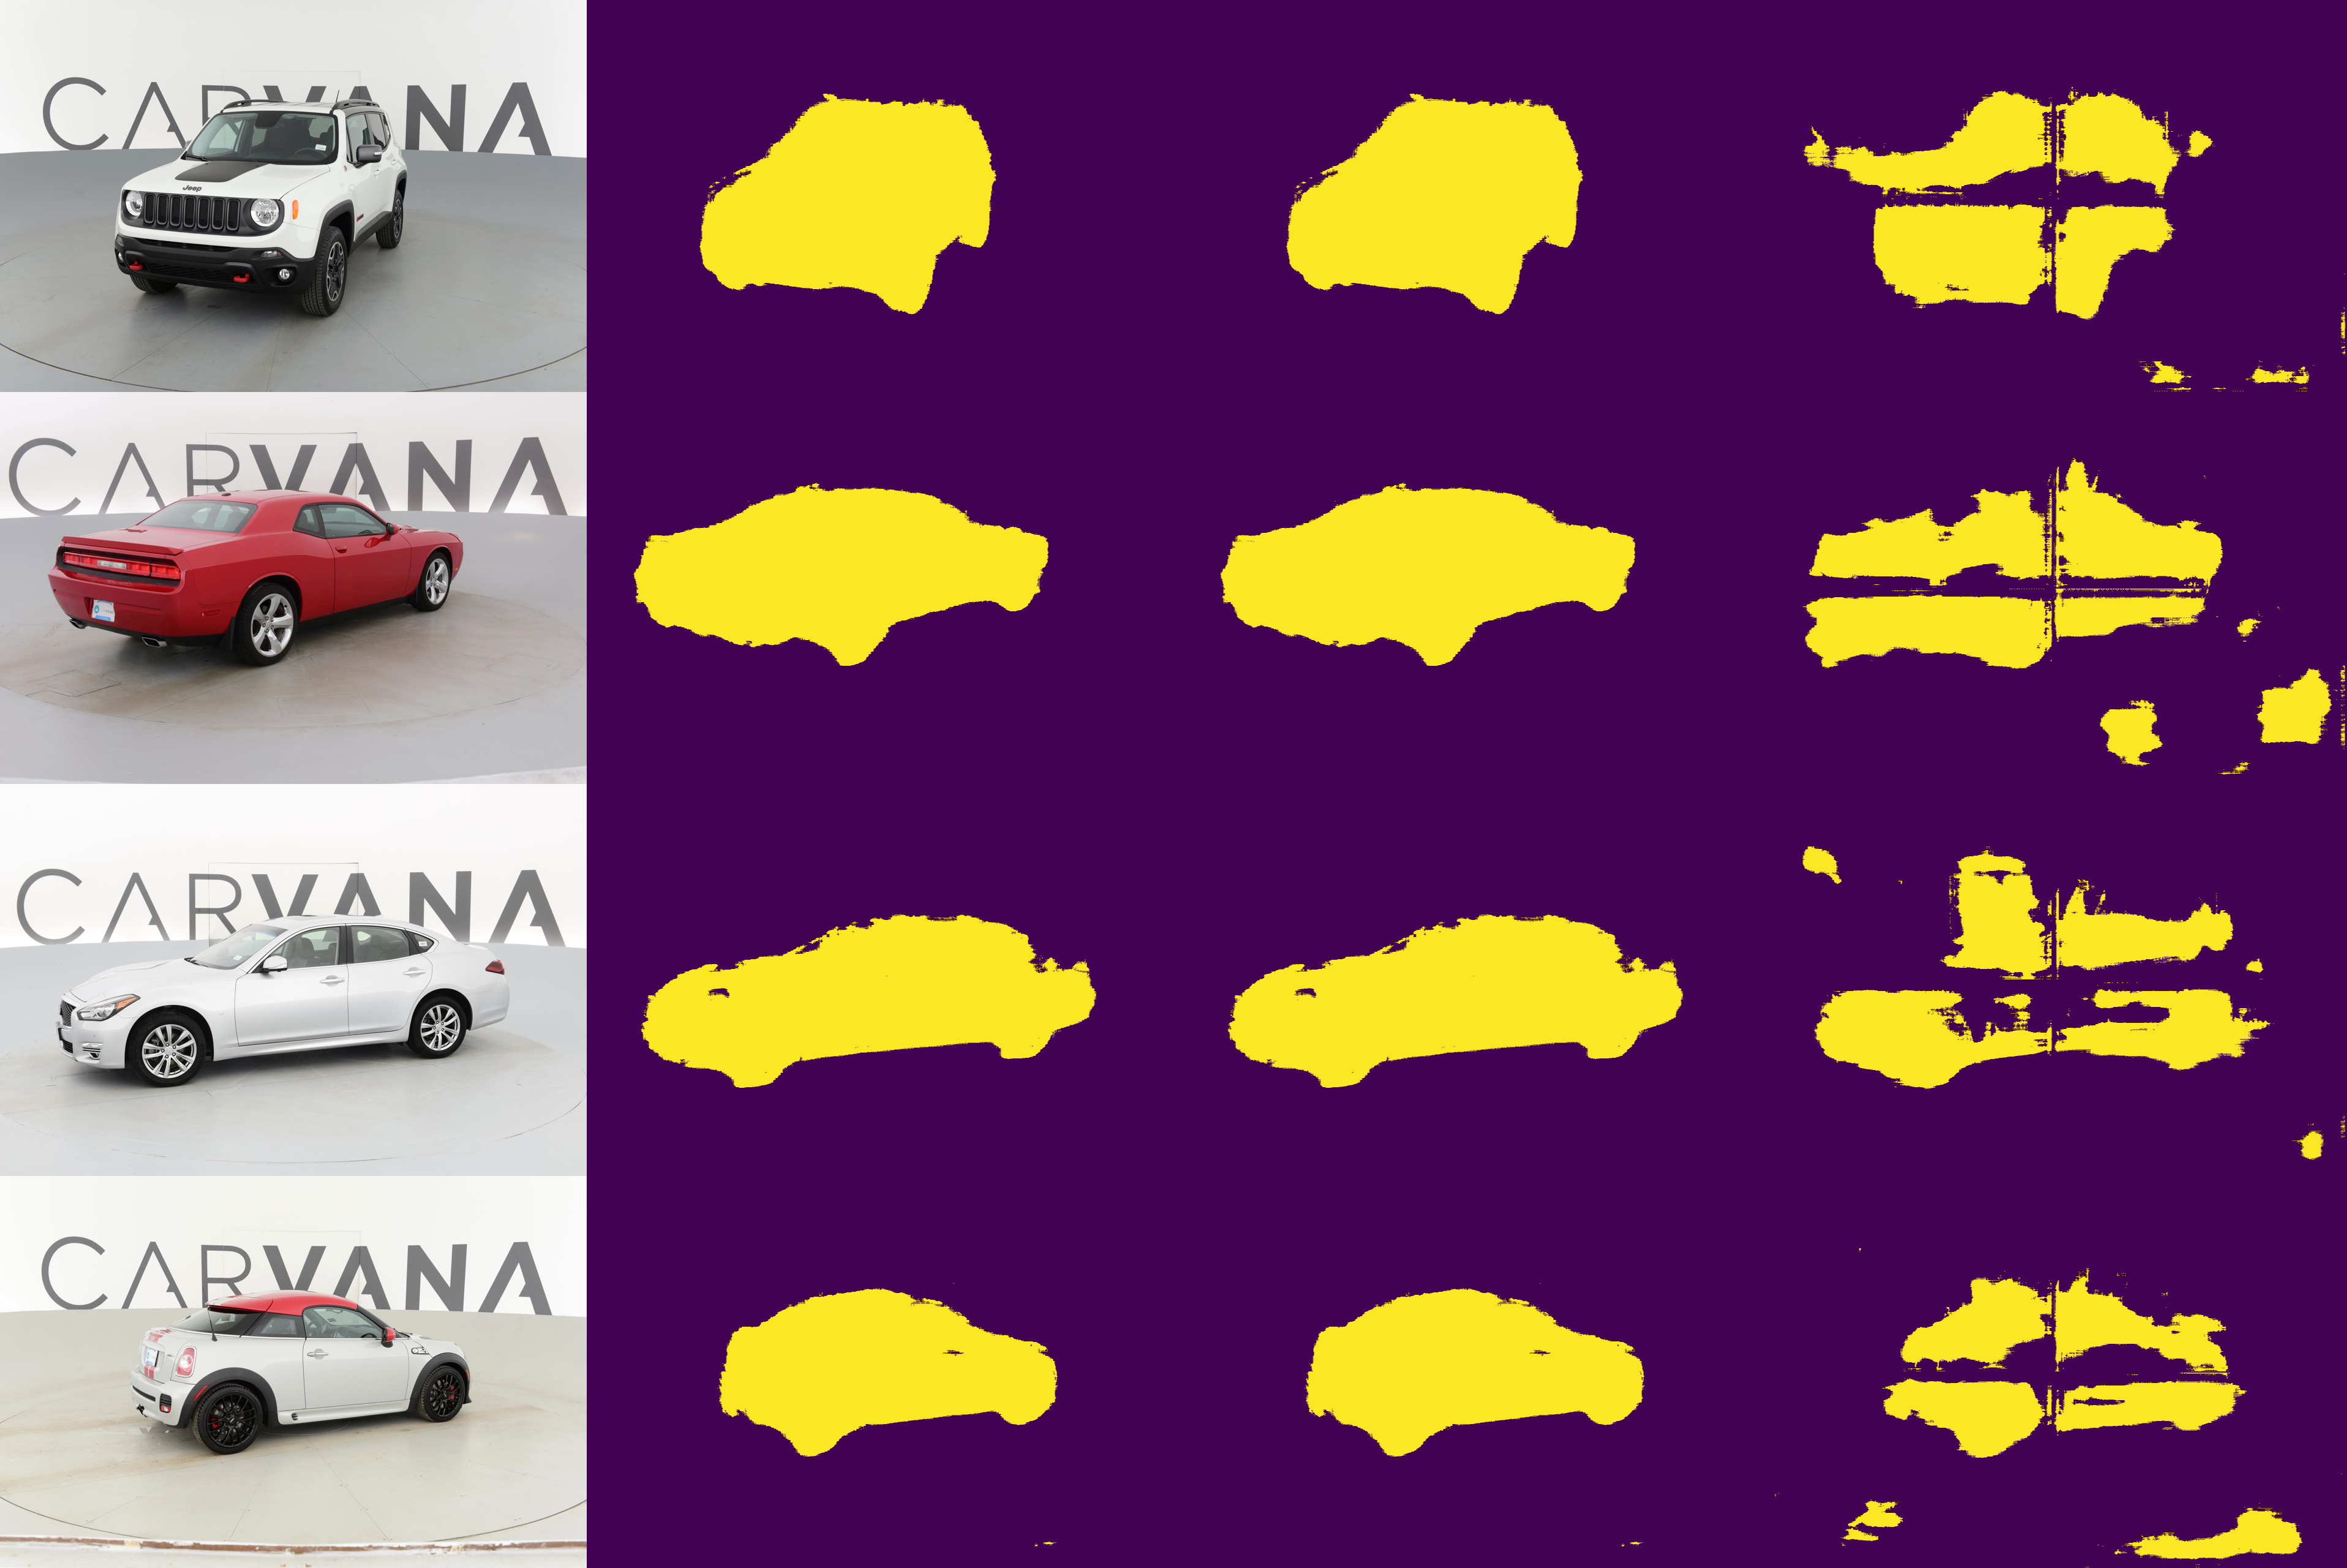
\includegraphics[width=1\linewidth]{figures/3_outputs.png}
	\caption{Comparison between Original Images and Outputs from Image Segmentation for Carvana Image Masking Challenge Dataset~\cite{brian2017carvanadataset} on an Android Phone: Uncompressed U-Net, FR Compressed and Decompressed U-Net, and FR Compressed and Decompressed U-Net Processing Four Parts of an Image Simultaneously.}
\end{figure}

The left-hand column of the ~\ref{image:3_outputs} shows the original images we want to implement the image segmentation. From left to right, the three columns represent three outputs generated by an Android phone respectively: output from non-compressed model, output from FR compressed model, output from FR compressed model with 4 parts. Table~\ref{table:ram_usage} illustrates the results among three ways of image segmentation. Table~\ref{table:ram_usage} shows that the average usages of RAM among three experiments are 3.2687 GB, 1.9318 GB, and 1.3063 GB respectively. It is obvious that Frequency Regularization on Android decreases the usage of RAM significantly. Because of this, more Android phones with lower-end hardware can probably use these two algorithms. To analyze Table~\ref{table:dice_score}, the table illustrates the average dice scores among three experiments. For using the compressed model (i.e. FR) directedly, the dice score is 0.9718 which is the same as using the original non-compressed model. Moreover, for using the compressed model on four separated parts of the image, the dice score shows a small number of 0.7567, which means that the image segmentation under this algorithm does not have good quality. Combining these two tables: Table~\ref{table:ram_usage} and Table~\ref{table:dice_score}, using FR directedly on Android is the best algorithm to implement the U-Net. Moreover, Fig.~\ref{image:3_outputs} also tells us which algorithm has the best outcome. Obviously, the original model and compressed model by FR have almost the same quality of image segmentation. By visual perception, we are more certain that FR is a highly efficient algorithm even if the system is Android.


\section{Limitation}
\subsection{Incomplete Mobile PyTorch}
In some situations, some PyTorch features may still not work when running the code because of the difference in hardware structure between the computer and mobile devices~\cite{fojtik2022cpu}. For instance, the Discrete Fast Fourier Transforms, mobile devices do not support this operation due to the requirement of GPU involvement. Therefore, an alternative solution is to convert the tensor data to the NumPy array, which runs through the CPU. After the transformation, we then convert back to the PyTorch tensor array. Many functions require conversion to make it work in the Frequency Regularization algorithm.

\subsection{Unknown Trend}
\begin{figure}[h]
	\centering
	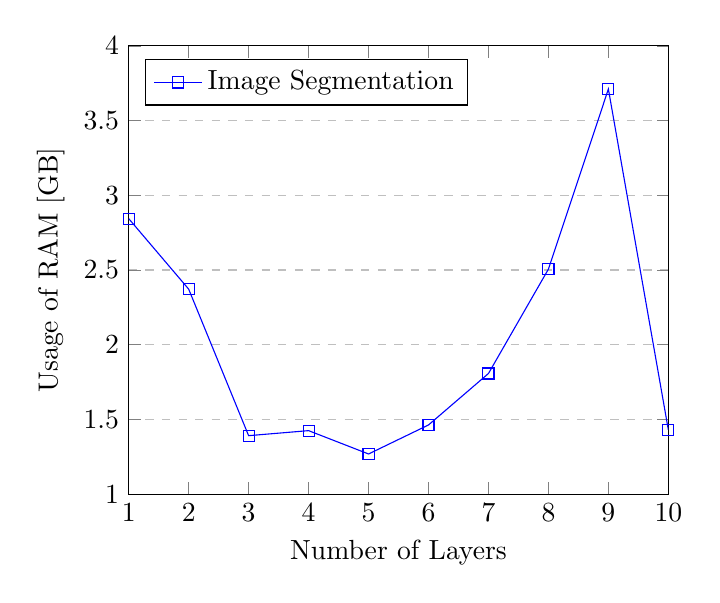
\begin{tikzpicture}
		\begin{axis}[
			xlabel={Number of Layers},
			ylabel={Usage of RAM [GB]},
			xmin=1, xmax=10,
			ymin=1, ymax=4,
			xtick={1,2,3,4,5,6,7,8,9,10},
			ytick={1,1.5,2,2.5,3,3.5,4},
			legend pos=north west,
			ymajorgrids=true,
			grid style=dashed,
			]
			
			\addplot[
			color=blue,
			mark=square,
			]
			coordinates {
				(1, 2.84366848)
				(2, 2.371833856)
				(3, 1.391190016)
				(4, 1.42483456)
				(5, 1.268662272)
				(6, 1.462788096)
				(7, 1.807253504)
				(8, 2.505711616)
				(9, 3.710410752)
				(10, 1.430171648)
			};
			\addlegendentry{Image Segmentation}
			
		\end{axis}
	\end{tikzpicture}
	\caption{Trend of One of the Three Experiments about Optimal Frequency Regularization (i.e. free RAM layer by layer) on RAM Usage for Image Segmentation.}
	\label{plot:optimal}
\end{figure}
Fig.~\ref{plot:optimal} shows me the trend of usages of RAM by using the optimal Frequency regularization (i.e. free RAM layer by layer). For the three experiments by using the same method, we always get the same trend. It is unexpected since we thought the usage of RAM should keep decreasing while layers going down. 




\section{Future Work}
The main purpose of our future work is to prove the general applicability of Frequency Regularization~\cite{zhao2023fr}. We plan to expand more neural network models like ResU-Net, SegNet, X-Net, and so on. We also plan to figure out why the trend of usage of RAM looks werid. Moreover, adjusting and improving Frequency Regularization to fit more tasks not only image segmentation is also the direction we want to explore.


\section{Conclusion} 
We proposed an optimal frequency regularization, freeing the usage of RAM layer-by-layer without any loss. This creative approach based on Zhao et al. 's frequency regularization solved some limitations and improved their work a lot. Moreover, this approach helped us deploy it on Android devices successfully and quickly. To some extent, by using the approach proposed by us, the popularization of using large and complex neuralworks on mobile devices will become possible.

\newpage
\bibliographystyle{plain}
\bibliography{ref}


\end{document}
